%%%%%%%%%%%%%%%%%%%%%%%%%%%
% Journal Article
% LaTeX Template
% Version 2.0 (February 7, 2023)
%
% This template originates from:
% https://www.LaTeXTemplates.com
%
% Author:
% Vel (vel@latextemplates.com)
%
% License:
% CC BY-NC-SA 4.0 (https://creativecommons.org/licenses/by-nc-sa/4.0/)
%
% NOTE: The bibliography needs to be compiled using the biber engine.
%
%%%%%%%%%%%%%%%%%%%%%%%%%%%%%%%%%%%%%%%%%

%----------------------------------------------------------------------------------------
%	PACKAGES AND OTHER DOCUMENT CONFIGURATIONS
%----------------------------------------------------------------------------------------

\documentclass[
	a4paper, % Paper size, use either a4paper or letterpaper
	11pt, % Default font size, can also use 11pt or 12pt, although this is not recommended
	unnumberedsections, % Comment to enable section numbering
	twoside, % Two side traditional mode where headers and footers change between odd and even pages, comment this option to make them fixed
]{LTJournalArticle}

\addbibresource{sample.bib} % BibLaTeX bibliography file

\runninghead{Building Blocks of a Microkernel} % A shortened article title to appear in the running head, leave this command empty for no running head

\footertext{\textit{Undergraduate Project Report} (2023)} % Text to appear in the footer, leave this command empty for no footer text

\setcounter{page}{1} % The page number of the first page, set this to a higher number if the article is to be part of an issue or larger work

%----------------------------------------------------------------------------------------
%	TITLE SECTION
%----------------------------------------------------------------------------------------

\title{Building Blocks of a Microkernel: \\ Lessons from seL4} % Article title, use manual lines breaks (\\) to beautify the layout

% Authors are listed in a comma-separated list with superscript numbers indicating affiliations
% \thanks{} is used for any text that should be placed in a footnote on the first page, such as the corresponding author's email, journal acceptance dates, a copyright/license notice, keywords, etc
\author{%
	\href{https://1-Harshit.github.io/}{Harshit Raj}\thanks{Supervised by: \href{https://www.cse.iitk.ac.in/users/deba/}{Prof. Debadatta Mishra}\\ \textbf{Submitted:} Apr 25, 2023}
}

% Affiliations are output in the \date{} command
\date{\footnotesize Department of Computer Science and Engineering \\ Indian Institute of Technology Kanpur}

% Full-width abstract
\renewcommand{\maketitlehookd}{%
	\begin{abstract}
		\noindent Lorem ipsum dolor sit amet, consectetur adipiscing elit. Praesent porttitor arcu luctus, imperdiet urna iaculis, mattis eros. Pellentesque iaculis odio vel nisl ullamcorper, nec faucibus ipsum molestie. Sed dictum nisl non aliquet porttitor. Etiam vulputate arcu dignissim, finibus sem et, viverra nisl. Aenean luctus congue massa, ut laoreet metus ornare in. Nunc fermentum nisi imperdiet lectus tincidunt vestibulum at ac elit. Nulla mattis nisl eu malesuada suscipit. Aliquam arcu turpis, ultrices sed luctus ac, vehicula id metus. Morbi eu feugiat velit, et tempus augue. Proin ac mattis tortor. Donec tincidunt, ante rhoncus luctus semper, arcu lorem lobortis justo, nec convallis ante quam quis lectus. Aenean tincidunt sodales massa, et hendrerit tellus mattis ac. Sed non pretium nibh. Donec cursus maximus luctus. Vivamus lobortis eros et massa porta porttitor.
	\end{abstract}
}

%----------------------------------------------------------------------------------------

\begin{document}

\maketitle % Output the title section

%----------------------------------------------------------------------------------------
%	ARTICLE CONTENTS
%----------------------------------------------------------------------------------------

\section{Introduction}

Kernel is a piece of code that serves as the core of an operating system. It manages the system's resources and provides a layer of abstraction between the hardware and software. The kernel is responsible for handling tasks such as memory management, process scheduling, device drivers, and input/output (I/O) operations. All these operations take place in a privileged mode, also know as kernel mode. On the other hand, programs operate in user mode which doesn't allow them to directly access hardware resources. Instead, they need to utilize the operating system to access these resources via different abstractions and interfaces.

Over the years this privileged code has increased with addition of newer technologies and this is as dangerous as useful. If any malitious access is allowed here that could compromise the entire system. This has occured on many mainstream system. Linux kernel comprises of 20 Million lines of source code, it is estimated that it contains tens of thousands of bugs \cite{Biggs:2018}. This idea is captured by saying that Linux has a large trusted computing base (TCB), which is defined as the subset of the overall system that must be trusted to operate correctly for the system to be secure~\cite{Heiser:2020}.

The idea behind a microkernel design is to drastically reduce the TCB to have a secure base to build a system. In a well-designed microkernel, such as seL4, it is of the order of ten thousand lines of source code. As seen in Figure~\ref{fig:microsemantic} the monolithic kernel structure provides every functionality from kernel mode, i.e.\ privileged mode making the TCB large. On the other hand, the microkernel structure provides only the bare minimum functionality from kernel mode and the rest of the functionality is provided by user mode programs. This makes the TCB small and secure. However the downside of this approach is that it requires a lot of user mode programs to be written to provide the functionality and this incurs a performance penalty.

In this report we will be looking at the building blocks of a microkernel and how they are implemented in seL4. We will also be looking at the a design to build a teching microkernel using gem5 simulator~\cite{gem5}. This report aims to explore the concept of microkernels and their significance in designing secure operating systems. A microkernel design addresses this problem by minimizing the TCB to only include the essential functions of the kernel. 

\begin{figure*} % Double column using figure`*`
	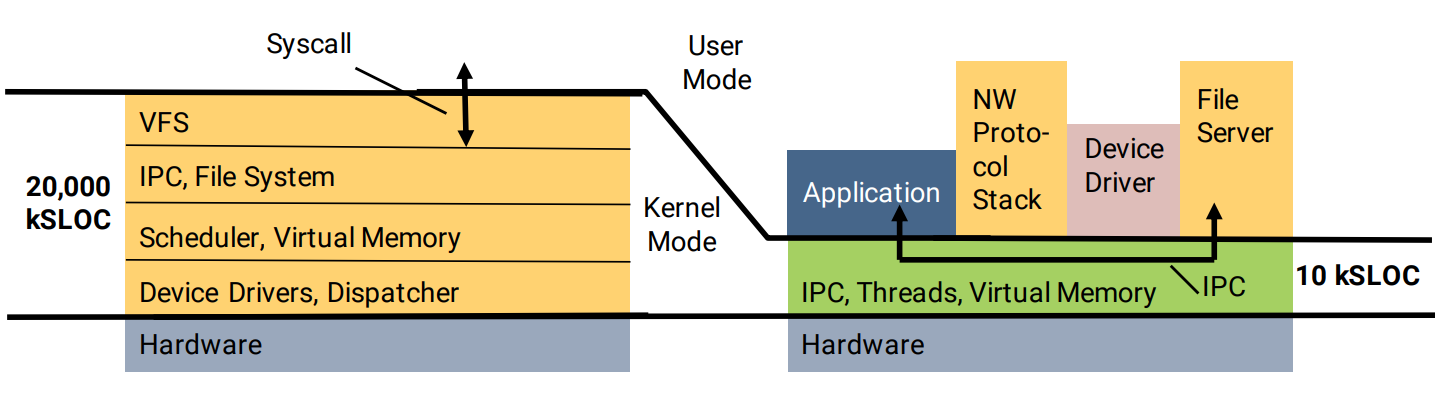
\includegraphics[width=\linewidth]{mono-vs-micro.png}
	\caption{To left is a monolithic structure and microkernel structure on right~\cite{Heiser:2020}}
	\label{fig:microsemantic}
\end{figure*}

\section{Microkernel Design}

The primary objective of Microkernels is to offer a small and secure kernel that is critical for security. The kernel provides only the essential functionality in kernel mode, and the remaining functionality is provided by user mode programs. This approach helps keep the Trusted Computing Base (TCB) small and secure, which reduces the attack surface. A well-designed microkernel, such as seL4, is typically only about ten thousand lines of source code, in contrast to the Linux kernel, which is approximately 20 million lines of code. This significant difference in size results in a much smaller TCB in a microkernel design, as shown in Figure~\ref{fig:microsemantic}. Let us now consider a microkernel design principle.

\subsection{Minimality \& Generality}

The principles of minimality and Inter-Process Communication (IPC) performance were the primary drivers of Liedtke's designs. He firmly believed that minimality enhances IPC performance. To express this idea, he introduced the microkernel \textit{minimality principle} as follows:~\cite{Liedtke:1995}

\begin{quote}
\textit{A concept is tolerated inside the µ-kernel only if moving it outside the kernel, i.e. permitting competing implementations, would prevent the implementation of the system's required functionality}
\end{quote}

L4 had an implicit driver for the design of kernel mechanisms, which was generality: the aim was to create a foundation on which various systems could be built, almost anything that could run on a processor powerful enough to provide protection.

However, none of the designers of L4 kernels to date claim that they have developed a ``pure'' microkernel that strictly adheres to the minimality principle. For instance, all of them have a scheduler in the kernel, which implements a specific scheduling policy, usually a hard-priority round-robin. To date, no one has been able to come up with a general in-kernel scheduler or a viable mechanism that delegates all scheduling policy to the user level without imposing a significant overhead.

In conclusion, microkernels maintain minimality as a crucial design principle and generality as the overall goal.~\cite{Heiser:2016}

\subsection{Building Blocks}

In this section, we will briefly examine the various building blocks that make up a microkernel.

\subsubsection{Components}

Unlike traditional operating systems, microkernels do not provide any typical OS services. Instead, microkernel designs use \textbf{user-mode} programs called components to provide necessary system services. For example, a file system component provides file system services. These components are loaded into the kernel and run in user mode. The kernel provides the Inter-Process Communication (IPC) mechanism for these components to communicate with each other. Even the \textbf{user application} is a component in this design, as depicted in Figure~\ref{fig:microsemantic}.

\subsubsection{Kernel Objects}

Microkernels also include a limited set of well-defined core kernel objects. These objects run in privileged mode and are responsible for providing basic services, including an entry point for interrupt handling, IPC, basic virtual memory management, thread management, and scheduling. These are the only functionalities provided by the kernel. The rest of the services are provided by the components, as shown in Figure~\ref{fig:microsemantic}.

\subsubsection{Build System}
As the components and kernel objects are complex and involved, they need to be configured before the system boots up and sent to appropriate locations in memory. This is the responsibility of the build system, which configures the components and kernel objects and sets metadata for the components.


\subsubsection*{} We will discuss each of these building blocks in more detail later.

%------------------------------------------------

% \section{Results}

% \begin{table} % Single column table
% 	\caption{Example single column table.}
% 	\centering
% 	\begin{tabular}{l l r}
% 		\toprule
% 		\multicolumn{2}{c}{Location} \\
% 		\cmidrule(r){1-2}
% 		East Distance & West Distance & Count \\
% 		\midrule
% 		100km & 200km & 422 \\
% 		350km & 1000km & 1833 \\
% 		600km & 1200km & 890 \\
% 		\bottomrule
% 	\end{tabular}
% 	\label{tab:distcounts}
% \end{table}

% Referencing a table using its label: Table\ref{tab:distcounts}.

% \begin{table*} % Full width table (notice the starred environment)
% 	\caption{Example two column table with fixed-width columns.}
% 	\centering % Horizontally center the table
% 	\begin{tabular}{L{0.2\linewidth} L{0.2\linewidth} R{0.15\linewidth}} % Manually specify column alignments with L{}, R{} or C{} and widths as a fixed amount, usually as a proportion of \linewidth
% 		\toprule
% 		\multicolumn{2}{c}{Location} \\
% 		\cmidrule(r){1-2}
% 		East Distance & West Distance & Count \\
% 		\midrule
% 		100km & 200km & 422 \\
% 		350km & 1000km & 1833 \\
% 		600km & 1200km & 890 \\
% 		\bottomrule
% 	\end{tabular}
% \end{table*}

\section{Components}

Components are user-mode programs that provide system services and also function as application programs. The kernel provides an Inter-Process Communication (IPC) mechanism for these components to communicate with each other, if permitted.

\subsection{Nature of Components:}
\begin{itemize}
\item Components are user-mode programs and do not possess special privileges. All logic is implemented in user mode, and components do not have access to kernel mode.
\item Components are independent of each other. If one component fails or is compromised, it does not affect the other components. The only impact is on the service provided by the failed component.
\item Components communicate with each other using the IPC mechanism provided by the kernel.
\item Components must be granted proper access rights at build time to access kernel objects, such as invoking IPC or accessing memory.
\item Components are configurable, allowing them to provide different services, interrupt handling, etc., at build time.
\item Components are reusable, meaning they can be used in different systems.
\end{itemize}

\subsection*{Representation of Components}
Components are represented as executables using Thread Control Blocks (TCBs). TCBs are data structures that contain information about the component and are used by the kernel to manage the component's execution. TCBs store information needed for context switching, scheduling, priority, IPC buffer, IPC call, capabilities, etc.

\subsubsection*{Data in TCB}
The TCB contains various information, including:
\begin{itemize}
\item Architecture-specific TCB state, such as the program counter and stack pointer.
\item Thread state: a three-word data structure indicating the current state of the component, which can be Inactive, Running, Restart, Blocked on Receive, Blocked on Send, Blocked on Reply, Blocked on Notification, or Idle Thread State.
\item Current fault of the component, i.e., the fault that caused the component to be blocked.
\item Maximum controlled priority of the component.
\item Scheduling context of the component, which contains scheduling parameters such as core and timeslice.
\item Scheduling and notification queues.
\end{itemize}

\subsection*{Capabilities}
Capabilities are access rights granted to components to access kernel objects. These access rights are determined at build time and are represented as a data structure in the kernel. Capabilities are configurable at build time and are used to invoke IPC, access memory, etc. Capabilities are essential for implementing the principle of least privilege and determine which component can access which interrupt.




\newpage

%----------------------------------------------------------------------------------------
%	 REFERENCES
%----------------------------------------------------------------------------------------

\printbibliography% Output the bibliography
\end{document}
